\newpage

\section{Projeto do controlador no MATLAB}

Função de transferência da planta:
\[
    G(s) = \frac{1}{s^2}
\]

Polos desejados:

\[
    s = -2 \pm 2j
\]


Root Locus sem o compensador:

\begin{figure}[H]
    \centering
    \caption{Root Locus com C(s) = 1.}
    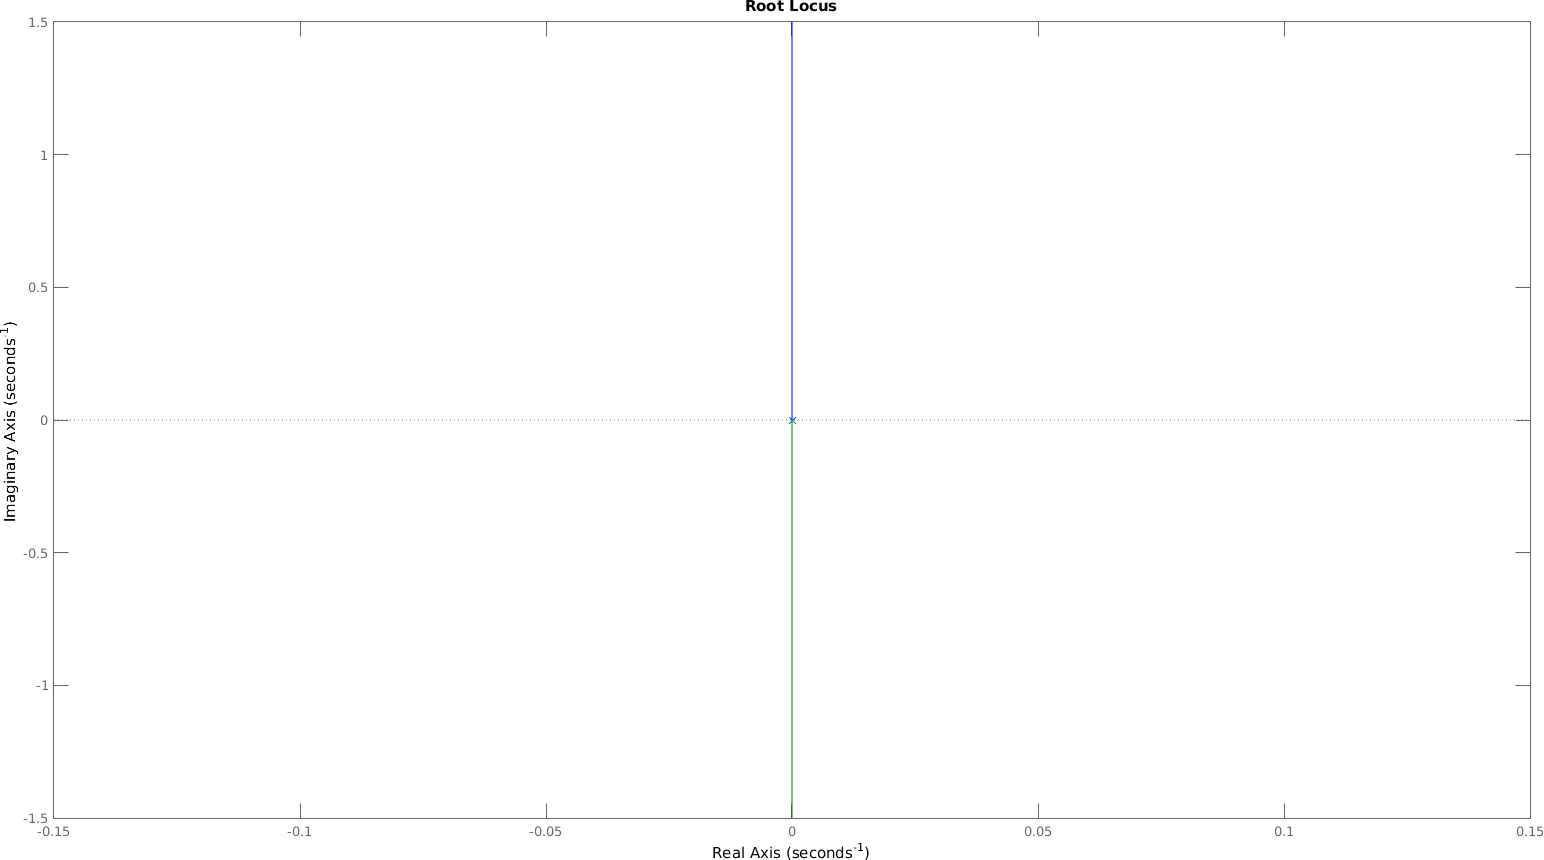
\includegraphics[scale=0.4]{rl_planta}
    \label{f_rl_planta}
\end{figure}


Ganho de fase desejado:
\[
    \Phi = atg-1(\frac{2}{2}) = 45 \degree.
\]

Como são 2 polos na origem, o ganho desejado é $90\degree$;

Calculando o zero e o polo para o compensador por avanço de fase:

\[
    Zero = 1.16
\]

\[
    Polo = 6.76
\]

Através da ferramenta RLTool do MATLAB foi encontrado o ganho do compensador:

\[
    Ganho = 19.0435
\]

A RL de malha fechada do sistema fica:

\begin{figure}[H]
    \centering
    \caption{Root Locus do sistema em malha fechada.}
    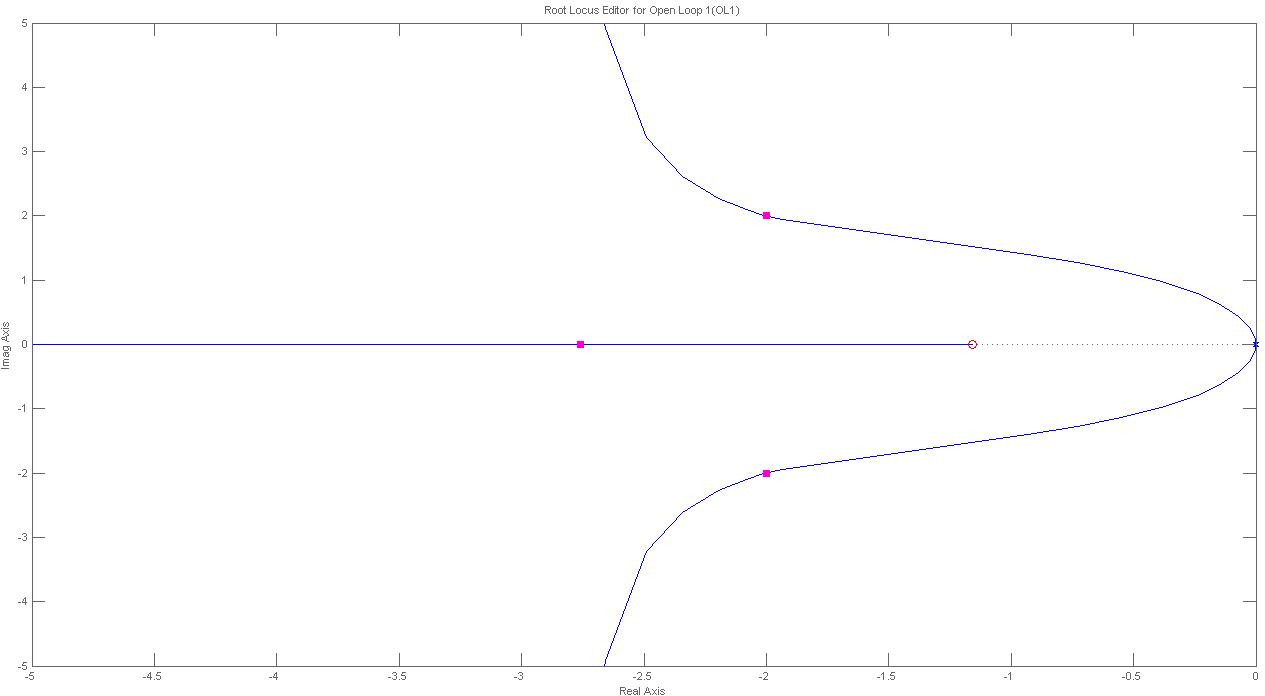
\includegraphics[scale=0.4]{rl}
    \label{f_rl}
\end{figure}

A resposta ao impulso é limitada, ou seja, o controlador é estável.
\begin{figure}[H]
    \centering
    \caption{Resposta ao impulso.}
    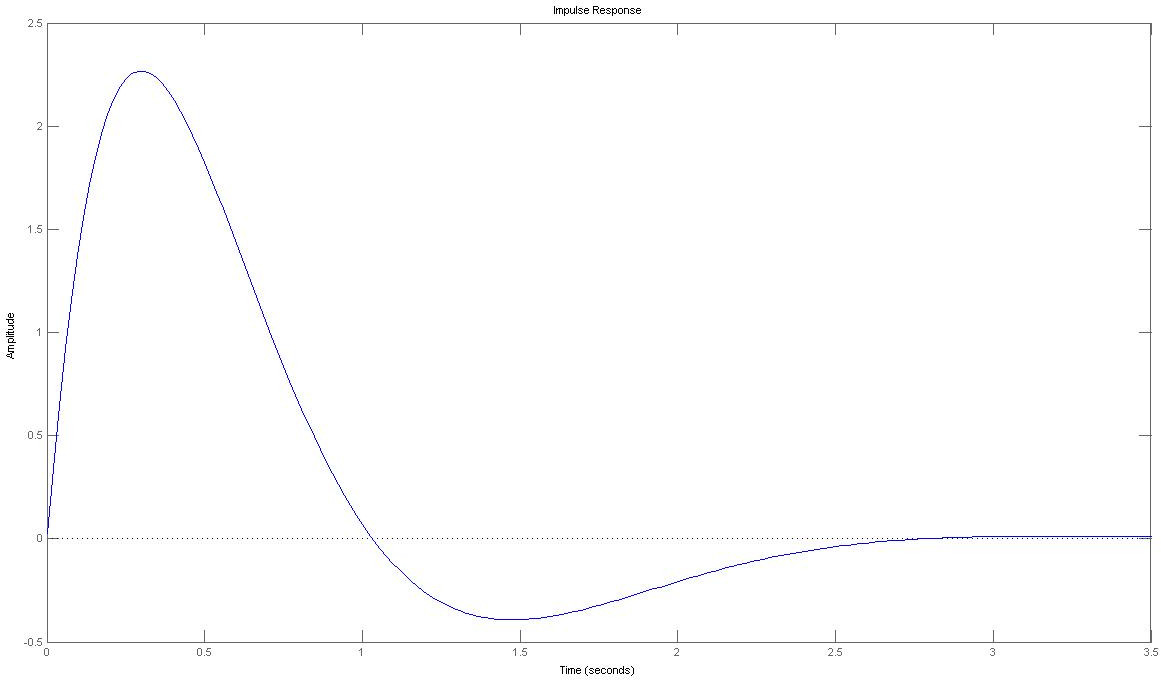
\includegraphics[scale=0.4]{imp}
    \label{f_imp}
\end{figure}

A resposta ao degrau é:
\begin{figure}[H]
    \centering
    \caption{Resposta do sistema a uma entrada do tipo degrau.}
    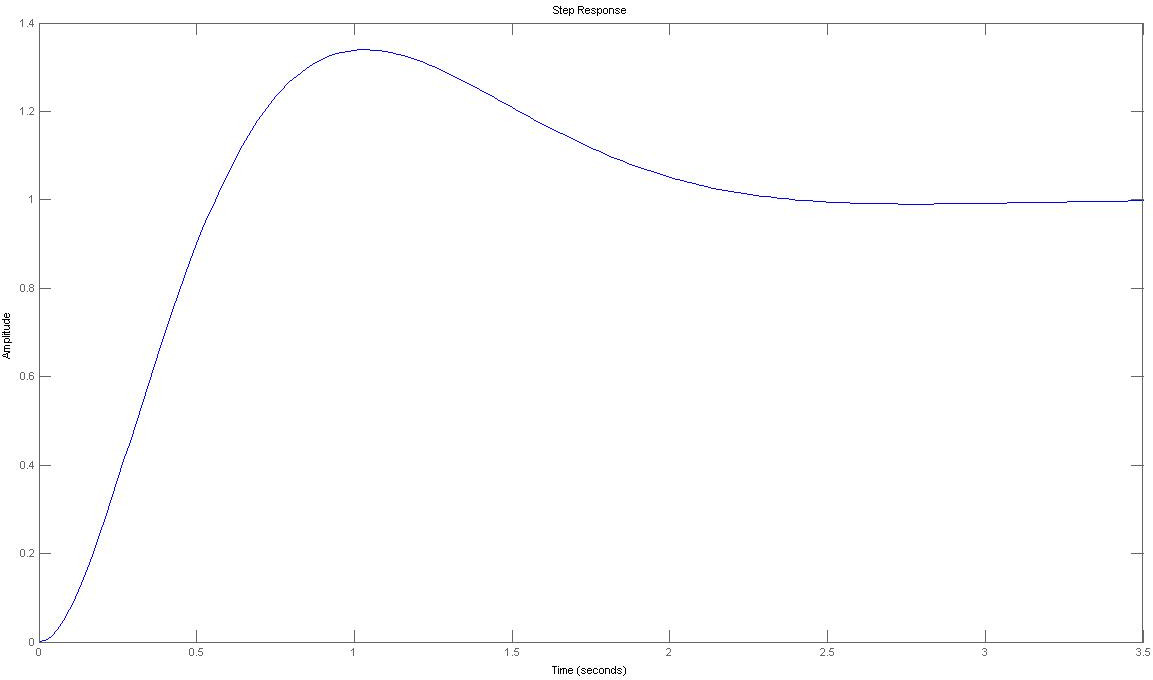
\includegraphics[scale=0.4]{step}
    \label{f_step}
\end{figure}


O circuito do compensador é:
\begin{figure}[H]
    \centering
    \caption{Controlador por avanço de fase feito com ampops.}
    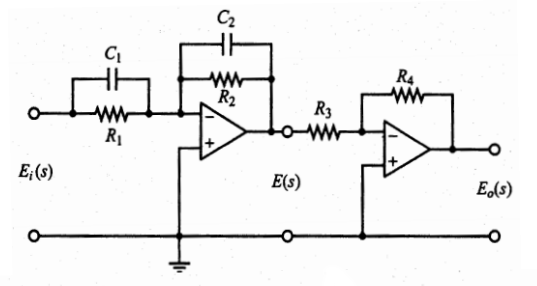
\includegraphics[scale=0.6]{sch_avanco}
    \label{f_sch_avanco}
\end{figure}


Calculando o valor de $R_1$ e $C_1$:

\[
    -\frac{1}{R_1C_1} = 1.16.
\]

Fazendo $R_1$ = $1 k\ohm$.
\[
    C_1 = \frac{1k}{1.16} = 65.5 \, \mu F.
\]


Calculando o valor de $R_2$ e $C_2$:
\[
    -\frac{1}{R_2C_2} = 6.76.
\]

Fazendo $R_2$ = $1 k\ohm$.
\[
C_2 = \frac{1k}{6.76} = 147.93 \, \mu F.
\]

Calculando o valor de $R_3$ e $R_4$:
\[
-\frac{R_4}{R_3} = 19.0435.
\]

Fazendo $R_3$ = $1 k\ohm$.
\[
R_4 = 1k\times 19.0435 = 19.0435  \, k \ohm.
\]

O circuito final montado no ORCAD é:
\begin{figure}[H]
    \centering
    \caption{Circuito do sistema.}
    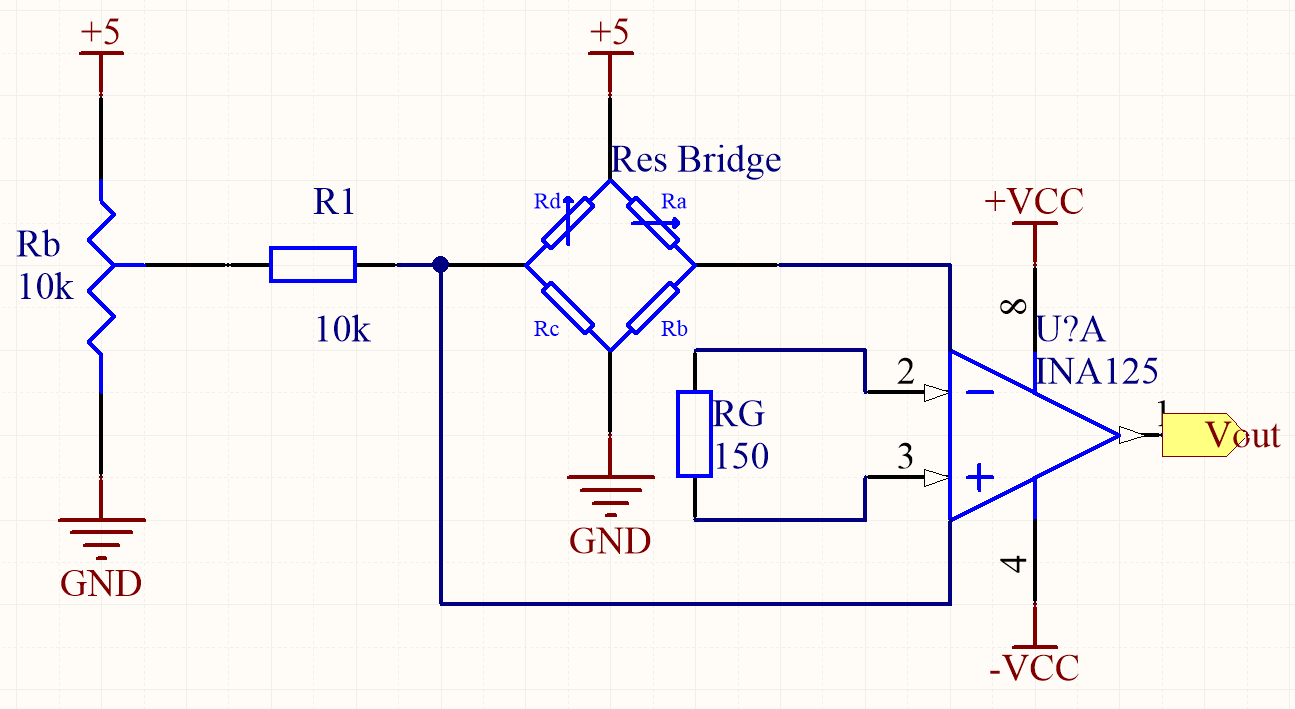
\includegraphics[scale=0.4]{sch}
    \label{f_sch}
\end{figure}

A saída do circuito fica:
\begin{figure}[H]
    \centering
    \caption{Saida do sistema.}
    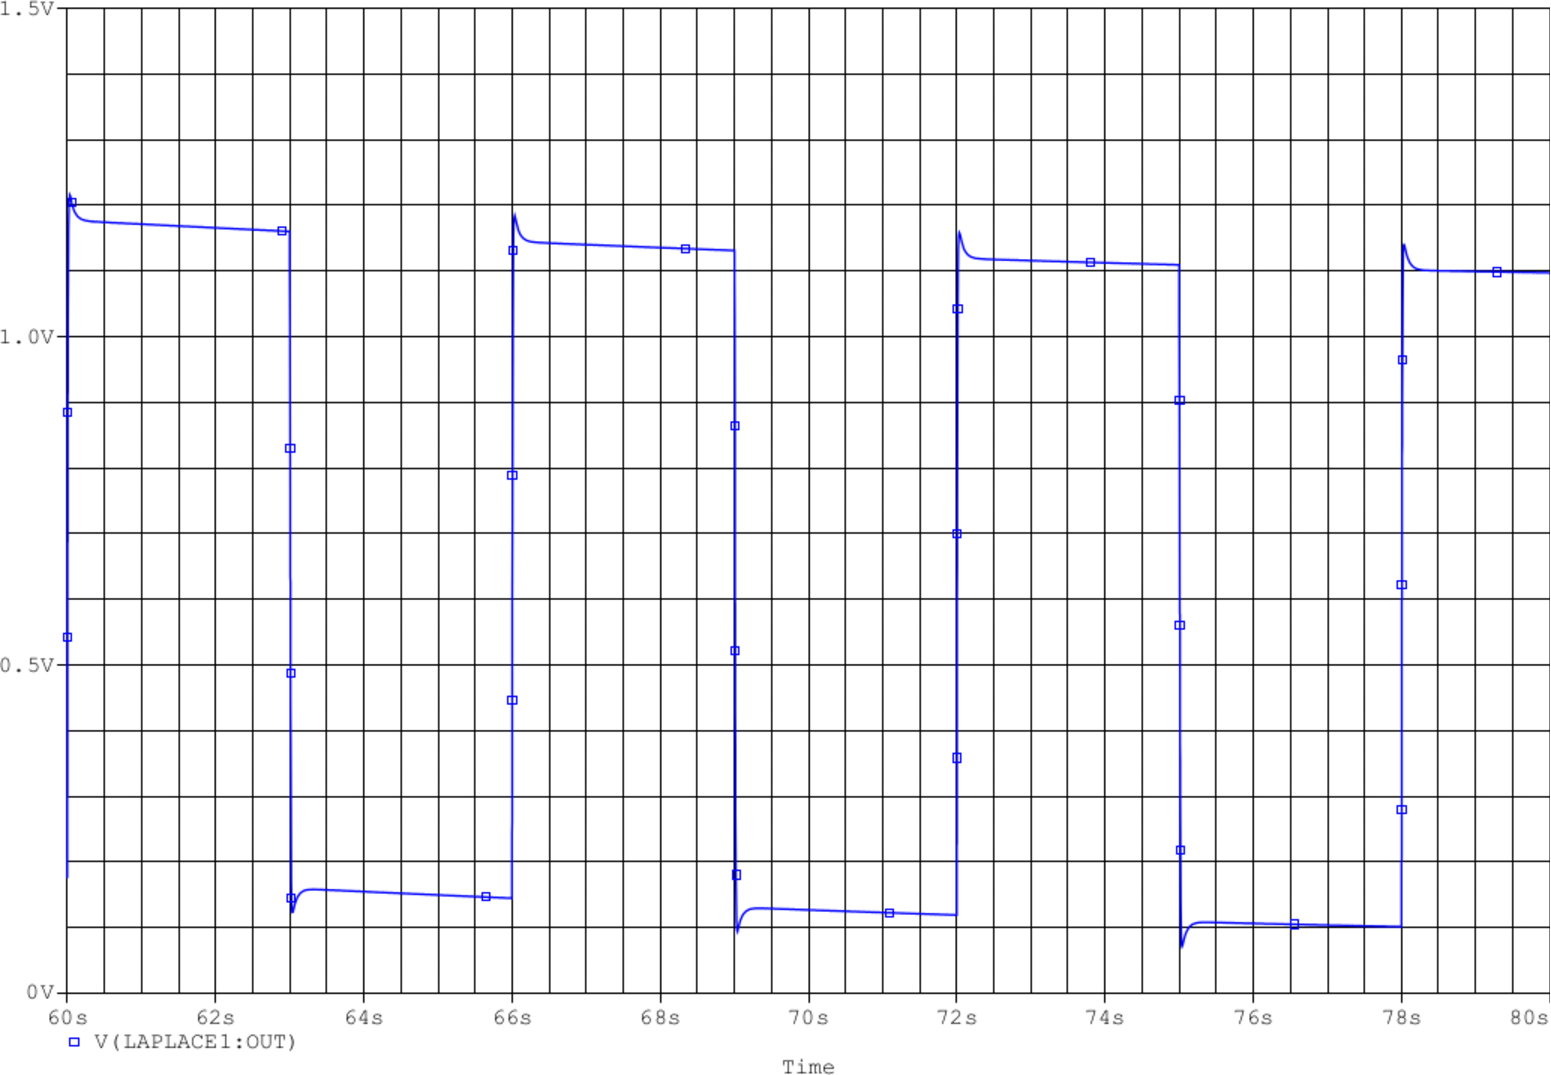
\includegraphics[scale=0.4]{saida}
    \label{f_saida}
\end{figure}

Com zoom:
\begin{figure}[H]
    \centering
    \caption{Zoom na borda.}
    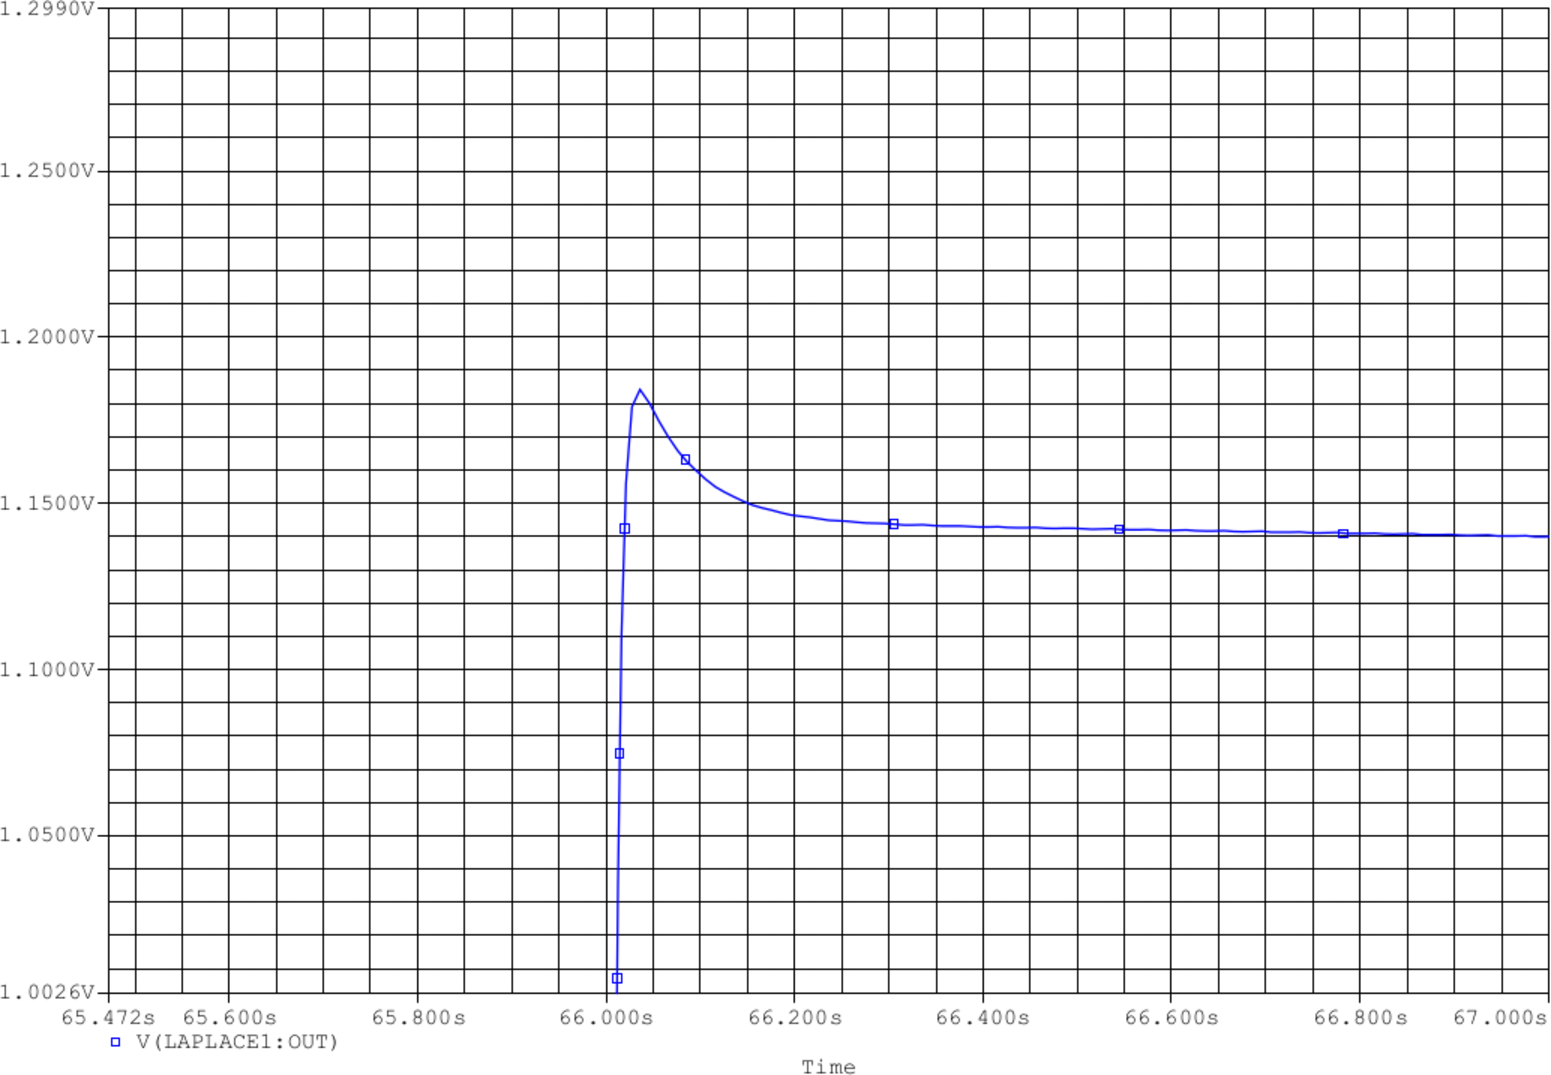
\includegraphics[scale=0.4]{saidazoom}
    \label{f_saidazoom}
\end{figure}


Note que a saída é praticamente igual a do MATLAB.
